\chapter{Αποτελέσματα}
Στο παρόν κεφάλαιο παρουσιάζονται τα αποτελέσματα των προσομοιώσεων και προγραμμάτων που υλοποιήθηκαν στα πλαίσια της διπλωματικής εργασίας. 
Η αναλυτική περιγραφή του τρόπου προσομοίωσης και υλοποίησης παρουσιάζεται στο Κεφάλαιο \ref{ch:simulation-methods}, ενώ η θεωρητική ανάλυση παρουσιάζεται στο Κεφάλαιο \ref{ch:theoretical-background}.
Επιγραμματικά, παρουσιάζονται:
\begin{itemize}
\item Τα αποτελέσματα της μελέτης επιρροής μεταβλητών σε έναν \en{Electron Beam Scanner} με βάση το θεωρητικό μοντέλο, όπως υλοποιήθηκε στο \en{MATLAB}
\item Τα αποτελέσματα της μελέτης επιρροής μεταβλητών σε έναν \en{Electron Beam Scanner}, όπως αυτός προσομοιώνεται στο \en{CST}
\item Τα αποτελέσματα της πλήρους προσομοίωσης ενός \en{Electron Beam Scanner} στο \en{CST} για πολλαπλές δέσμες
\item Τα αποτελέσματα της προσομοίωσης που χρησιμοποιεί το \en{CST} ως το μέσο υπολογισμού του ηλεκτρικού πεδίου της κύριας δέσμης και στη συνέχεια το \en{MATLAB} για τον υπολογισμό των τροχιών των σωματιδίων της δέσμης ανίχνευσης μέσα στο πεδίο που εξάγεται από το \en{CST}
\end{itemize}

\section{Επίδραση παραμέτρων του επιταχυντή στην ανίχνευση της δέσμης}
Στην ενότητα αυτή θα δούμε τα αποτελέσματα της επιρροής των παραμέτρων που αναφέρθηκαν στα στοιχεία της χαρακτηριστικής έλλειψης της δέσμης.
Οι παράμετροι που εξετάστηκαν επαναλαμβάνονται εδώ για τη διευκόλυνση του αναγνώστη:
\begin{enumerate}
	\item Ένταση της κύριας δέσμης $Q_i$ (ανά παλμό)
	\item Μήκος της κύριας δέσμης $\sigma$
	\item Αρχική θέση ριπής $\rho$ κατά $Y$
	\item Τάση της δέσμης ανίχνευσης $V$
\end{enumerate}

Η μελέτη της επιρροής των παραμέτρων έγινε αρχικά με υλοποίηση του μοντέλου που παρουσιάστηκε στην Υπο-Ενότητα \ref{sub:EBS-model} στο \en{MATLAB}.
Στη συνέχεια εξετάστηκε η επιρροή των ίδιων μεγεθών στο προσομοιωτικό περιβάλλον του \en{CST}.

\subsection{Αποτελέσματα μελέτης θεωρητικού μοντέλου στο \en{MATLAB}}

Αρχικά υπολογίστηκε και παρουσιάζεται η γραφική απεικόνιση της χαρακτηριστικής έλλειψης στις αρχικές τιμές των παραμέτρων.
Η χαρακτηριστική έλλειψη, όπως προκύπτει από τη χρήση των αρχικών τιμών των παραμέτρων (Πίνακας \ref{tab:simulation-initial-values}) παρουσιάζεται στο Σχήμα \ref{fig:MATLAB-initial-ellipse}.

\begin{figure}[tph]	
	\begin{subfigure}{0.47\textwidth}
		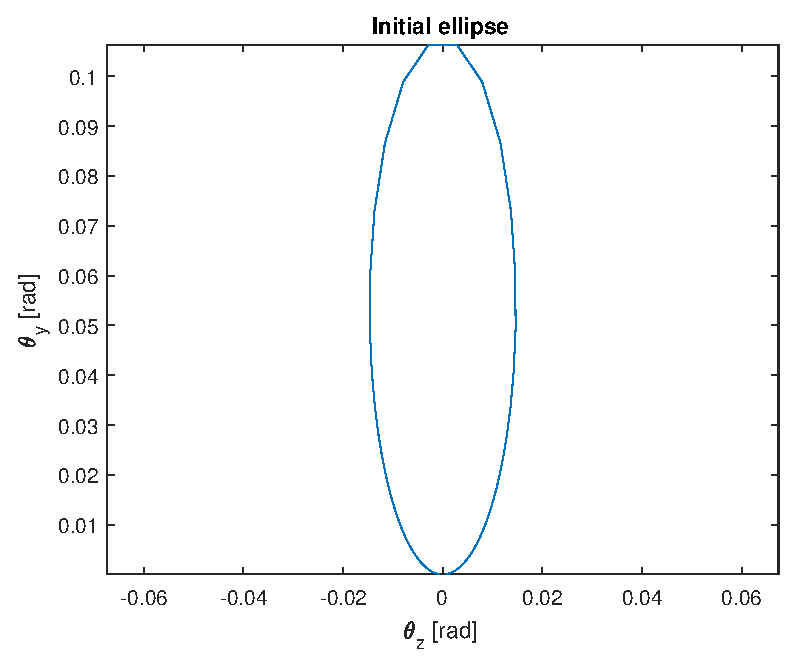
\includegraphics[width=\linewidth]{figures/MATLAB-variable-analysis/initial-ellipse}
		\centering
		\caption{Η χαρακτηριστική έλλειψη στην αρχική κατάσταση.}
		\label{fig:MATLAB-variable-analysis-initial-ellipse}
	\end{subfigure}
	\hfill
	\begin{subfigure}{0.47\textwidth}
		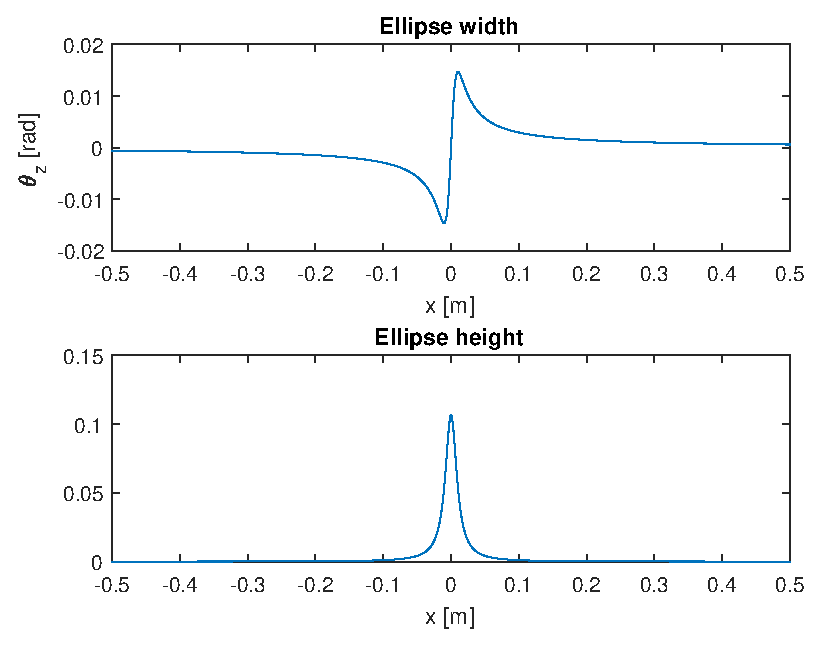
\includegraphics[width=\linewidth]{figures/MATLAB-variable-analysis/initial-ellipse-height-width}
		\centering
		\caption{Το πλάτος και ύψος της χαρακτηριστικής έλλειψης στην αρχική κατάσταση.}
		\label{fig:MATLAB-variable-analysis-initial-ellipse-height-width}
	\end{subfigure}
\caption{Απεικόνιση και στοιχεία της χαρακτηριστικής έλλειψης στην αρχική κατάσταση.}
\label{fig:MATLAB-initial-ellipse}
\end{figure}

Στη συνέχεια, υπολογίστηκε και παρουσιάζεται ο τρόπος επιρροής των παραμέτρων που αναφέρθηκαν, στο εύρος τιμών του Πίνακα \ref{tab:simulation-ranges}.


\begin{figure}[tph]	
	\centering
	\begin{subfigure}{0.47\textwidth}
		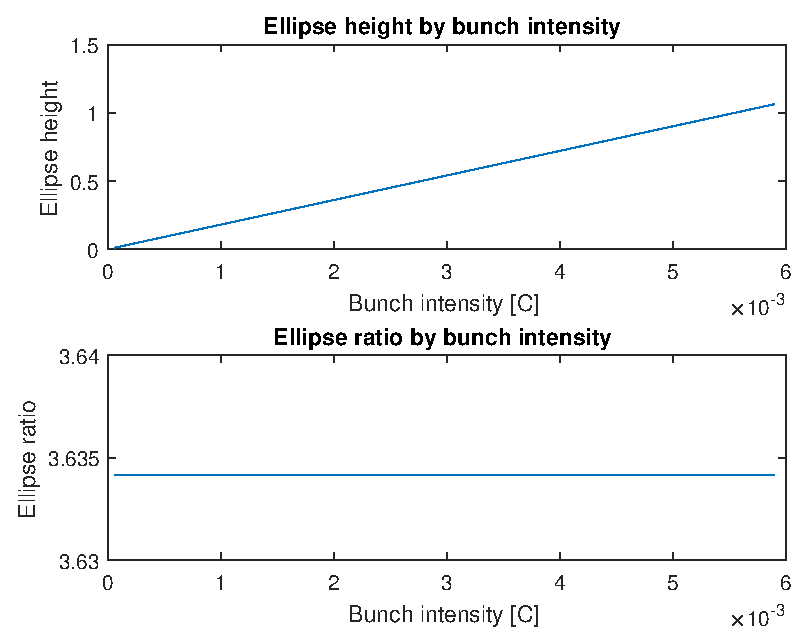
\includegraphics[width=\linewidth]{figures/MATLAB-variable-analysis/EBS-variables-intensity}
		\centering
		\caption{Επιρροή της έντασης της κύριας δέσμης στο ύψος και το λόγο της έλλειψης, με βάση το μαθηματικό μοντέλο.}
		\label{fig:EBS-variables-intensity}
	\end{subfigure}
	\hfill
	\begin{subfigure}{0.47\textwidth}
		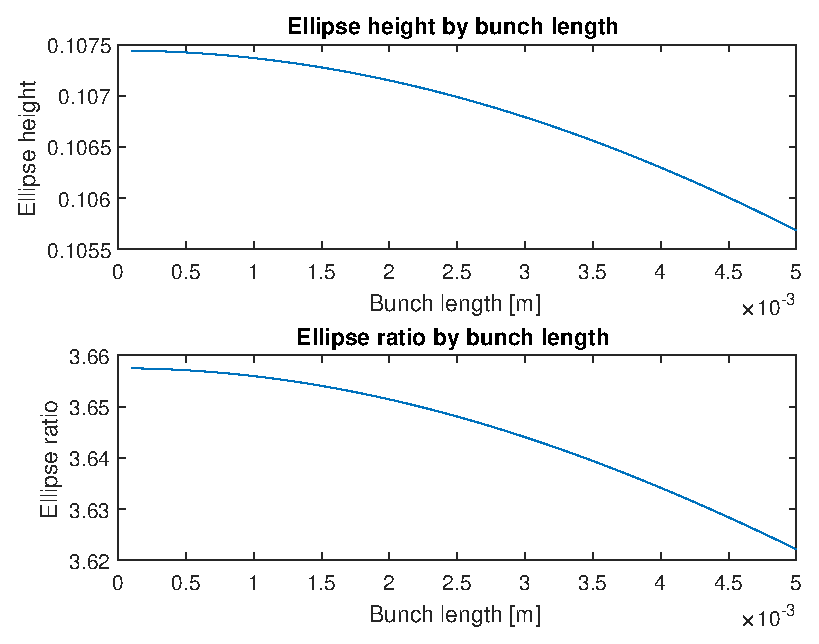
\includegraphics[width=\linewidth]{figures/MATLAB-variable-analysis/EBS-variables-length}
		\centering
		\caption{Επιρροή του μήκους της κύριας δέσμης στο ύψος και το λόγο της έλλειψης, με βάση το μαθηματικό μοντέλο.}
		\label{fig:EBS-variables-length}
	\end{subfigure}
	\par\bigskip
	\begin{subfigure}{0.47\textwidth}
		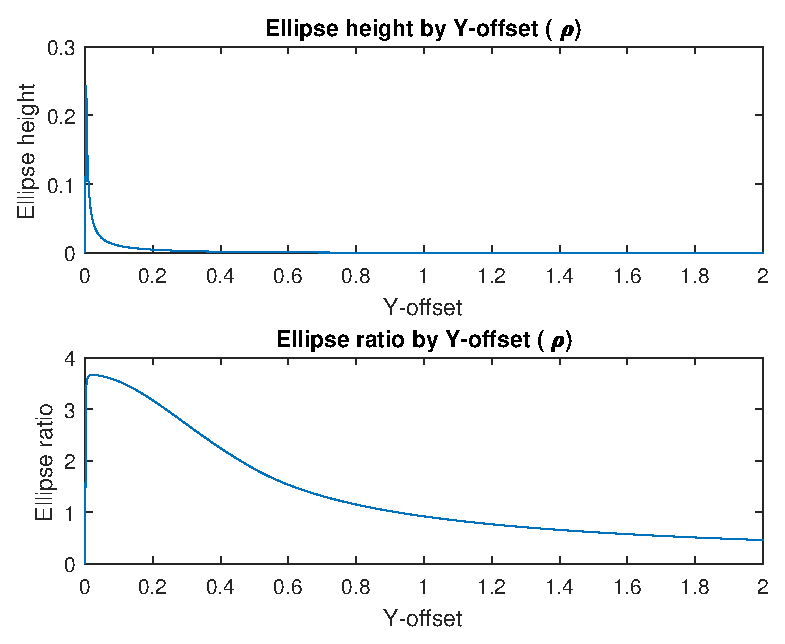
\includegraphics[width=\linewidth]{figures/MATLAB-variable-analysis/EBS-variables-rho}
		\centering
		\caption{Επιρροή της αρχικής θέσης ριπής ($Y$-\en{offset}) της δέσμης ανίχνευσης στο ύψος και το λόγο της έλλειψης, με βάση το μαθηματικό μοντέλο.}
		\label{fig:EBS-variables-rho}
	\end{subfigure}
	\hfill
	\begin{subfigure}{0.47\textwidth}
		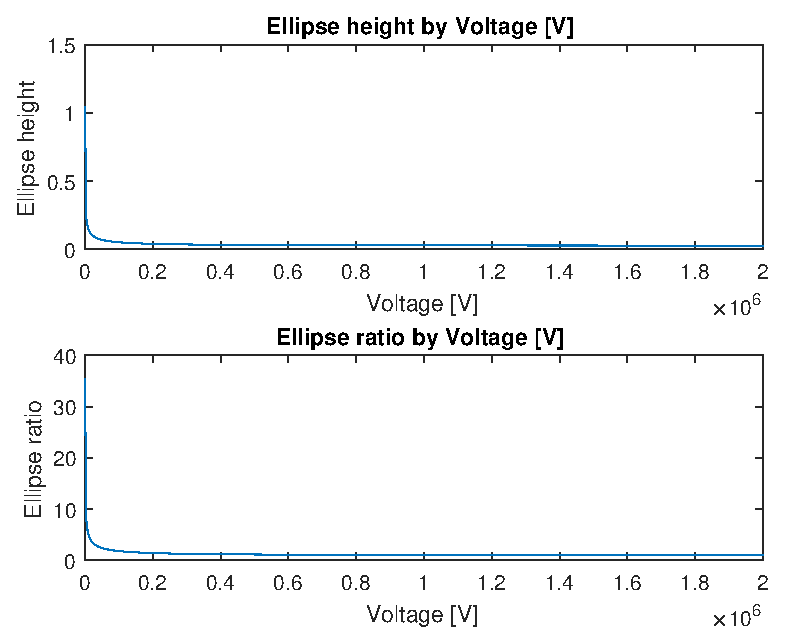
\includegraphics[width=\linewidth]{figures/MATLAB-variable-analysis/EBS-variables-voltage-linear}
		\centering
		\caption{Επιρροή της διαφοράς δυναμικού της κύριας δέσμης στο ύψος και το λόγο της έλλειψης, με βάση το μαθηματικό μοντέλο.}
		\label{fig:EBS-variables-voltage-linear}
	\end{subfigure}
\caption{Παρουσίαση της επιρροής των παραμέτρων στο πλάτος και το λόγο της έλλειψης, σύμφωνα με το θεωρητικό μοντέλο, όπως υλοποιήθηκε στο \en{MATLAB}.}	
\label{fig:EBS-MATLAB-variables}
\end{figure}

Από το Σχήμα \ref{fig:EBS-MATLAB-variables} μπορεί κανείς να παρατηρήσει τα εξής:
\begin{itemize}
\item Η ένταση της δέσμης έχει γραμμική σχέση με το ύψος της έλλειψης, αλλά ο λόγος δεν επηρεάζεται, και άρα δεν εξαρτάται από αυτήν.
\item Όσο αυξάνεται το μήκος της κύριας δέσμης μειώνεται το ύψος της έλλειψης.
Μειώνεται επίσης και ο λόγος της έλλειψης, αλλά πολύ λιγότερο.
\item Η αύξηση της αρχικής θέσης ριπής οδηγεί σε ραγδαία μείωση του ύψους και του λόγου της έλλειψης.
\item Η τάση της κύριας δέσμης προκαλεί μείωση του ύψους και λόγου της έλλειψης, για μικρές τιμές της. 
Μετά τα \SI{3e5}{\kilo \volt} περίπου η επιπλέον αύξηση της τάσης δεν προκαλεί αλλαγές στην έλλειψη.
\end{itemize}


\subsection{Αποτελέσματα προσομοίωσης στο \en{CST}}

Όμοια με παραπάνω, αρχικά υπολογίστηκε και παρουσιάζεται η γραφική απεικόνιση της χαρακτηριστικής έλλειψης στις αρχικές τιμές των παραμέτρων.
Η χαρακτηριστική έλλειψη, όπως προκύπτει από τη χρήση των αρχικών τιμών των παραμέτρων (Πίνακας \ref{tab:simulation-initial-values}) παρουσιάζεται στο Σχήμα \ref{fig:CST-initial-ellipse}.

\begin{figure}[tph]	
\centering
	\begin{subfigure}{0.7\textwidth}
		\includegraphics[width=\linewidth]{figures/CST-variable-analysis/CST-initial-ellipse}
		\centering
		\caption{Η χαρακτηριστική έλλειψη στην αρχική κατάσταση.}
		\label{fig:CST-variable-analysis-initial-ellipse}
	\end{subfigure}
	~
	\begin{subfigure}{0.47\textwidth}
		\includegraphics[width=\linewidth]{figures/CST-variable-analysis/CST-initial-ellipse-height}
		\centering
		\caption{Το ύψος της χαρακτηριστικής έλλειψης στην αρχική κατάσταση.}
		\label{fig:CST-variable-analysis-initial-ellipse-height}
	\end{subfigure}
	\hfill
	\begin{subfigure}{0.47\textwidth}
		\includegraphics[width=\linewidth]{figures/CST-variable-analysis/CST-initial-ellipse-width}
		\centering
		\caption{Το πλάτος της χαρακτηριστικής έλλειψης στην αρχική κατάσταση.}
		\label{fig:CST-variable-analysis-initial-ellipse-width}
	\end{subfigure}	
\caption{Έλλειψη και στοιχεία της στην αρχική κατάσταση, υπολογισμένα στο \en{CST}.}
\label{fig:CST-initial-ellipse}
\end{figure}

Παρατηρούμε ότι η έλλειψη έχει μια μικρή θετική περιστροφή, λόγω του ότι το πλάτος της χαρακτηριστικής έλλειψης στο Σχήμα \ref{fig:CST-initial-ellipse} (\subref{fig:CST-variable-analysis-initial-ellipse-width}) παρουσιάζει ελάχιστο για τιμή μεγαλύτερη (κατά απόλυτη τιμή) από την τιμή για την οποία παρουσιάζει μέγιστο.

Στη συνέχεια, παρουσιάζονται οι επιρροές των μεταβολών των μεταβλητών στο ύψος και το λόγο της έλλειψης.

\begin{figure}[tph]	
	\centering
	\begin{subfigure}{0.47\textwidth}
		\includegraphics[width=\linewidth]{figures/CST-variable-analysis/combined/CST-ellipse-height-ratio-by-bunch-intensity}
		\centering
		\caption{Επιρροή της έντασης της κύριας δέσμης στο ύψος και το λόγο της έλλειψης, στο περιβάλλον προσομοίωσης.}
		\label{fig:CST-ellipse-height-ratio-by-bunch-intensity}
	\end{subfigure}
	\hfill
	\begin{subfigure}{0.47\textwidth}
		\includegraphics[width=\linewidth]{figures/CST-variable-analysis/combined/CST-ellipse-height-ratio-by-bunch-length}
		\centering
		\caption{Επιρροή του μήκους της κύριας δέσμης στο ύψος και το λόγο της έλλειψης, στο περιβάλλον προσομοίωσης.}
		\label{fig:CST-ellipse-height-ratio-by-bunch-length}
	\end{subfigure}
	\par\bigskip
	\begin{subfigure}{0.47\textwidth}
		\includegraphics[width=\linewidth]{figures/CST-variable-analysis/combined/CST-ellipse-height-ratio-by-vertical-offset}
		\centering
		\caption{Επιρροή της αρχικής θέσης ριπής ($Y$-\en{offset}) της δέσμης ανίχνευσης στο ύψος και το λόγο της έλλειψης, στο περιβάλλον προσομοίωσης.}
		\label{fig:CST-ellipse-height-ratio-by-vertical-offset}
	\end{subfigure}
	\hfill
	\begin{subfigure}{0.47\textwidth}
		\includegraphics[width=\linewidth]{figures/CST-variable-analysis/combined/CST-ellipse-height-ratio-by-voltage}
		\centering
		\caption{Επιρροή της διαφοράς δυναμικού της κύριας δέσμης στο ύψος και το λόγο της έλλειψης, στο περιβάλλον προσομοίωσης.}
		\label{fig:CST-ellipse-height-ratio-by-voltage}
	\end{subfigure}
\caption[Όμοια με το Σχήμα \ref{fig:EBS-MATLAB-variables}, παρουσίαση της επιρροής των παραμέτρων στο πλάτος και το λόγο της έλλειψης στο περιβάλλον προσομοίωσης του \en{CST} αυτή τη φορά.]
{Παρουσίαση της επιρροής των παραμέτρων στο πλάτος και το λόγο της έλλειψης στο περιβάλλον προσομοίωσης του \en{CST}.}
\label{fig:EBS-CST-variables}
\end{figure}


Από το Σχήμα \ref{fig:EBS-CST-variables} μπορεί κανείς να παρατηρήσει τα εξής:
\begin{itemize}
\item Η ένταση της δέσμης έχει γραμμική σχέση με το ύψος της έλλειψης. 
Έχει επίσης γραμμική σχέση με το λόγο της έλλειψης, αλλά η κλίση της καμπύλης είναι σημαντικά μικρότερη.
\item Με εξαίρεση τα πρώτα δείγματα, όσο αυξάνεται το μήκος της κύριας δέσμης μειώνεται το ύψος της έλλειψης.
Ο λόγος της έλλειψης μειώνεται επίσης ως ένα σημείο όπου παρουσιάζει ελάχιστο, και στη συνέχεια αυξάνεται.
\item Η αύξηση της αρχικής θέσης ριπής οδηγεί στην αδυναμία μέτρησης, καθώς μειώνεται η επιρροή της κύριας δέσμης στη δέσμη ανίχνευσης.
Βλέπουμε ότι ο λόγος της έλλειψης στο Σχήμα \ref{fig:EBS-CST-variables} (\subref{fig:CST-ellipse-height-ratio-by-vertical-offset}) σταματά να έχει δείγματα μετά τα πρώτα 2, γι' αυτό και έχει σημειωθεί με κόκκινο χρώμα.
Επίσης, το ύψος της δέσμης παίρνει τιμές που δεν έχουν νόημα.
Αυτό γίνεται διότι η απόκλιση κατά $Z$ είναι μηδενική, με αποτέλεσμα να ισχύει $\theta_z = 0$ και να απειρίζεται ο λόγος.
\item Η τάση της κύριας δέσμης προκαλεί μείωση του ύψους και λόγου της έλλειψης, για μικρές τιμές της. 
Μετά τα περίπου \SI{5e8}{\volt}, η τάση της κύριας δέσμης πρακτικά δεν προκαλεί καμία επίδραση τόσο στο ύψος όσο και στο λόγο της έλλειψης.
\end{itemize}


\subsection{Σύγκριση αποτελεσμάτων}

Η σύγκριση των αποτελεσμάτων που παρουσιάστηκαν στις προηγούμενες ενότητες μας οδηγούν στις εξής παρατηρήσεις:

\begin{itemize}
\item Η ένταση της δέσμης στο μαθηματικό μοντέλο καθώς και στην προσομοίωση έχει γραμμική σχέση με το ύψος της έλλειψης. 
Όσον αφορά το λόγο της έλλειψης, αν και στο μαθηματικό μοντέλο δεν υπάρχει καμία επιρροή, προσομοίωση υπάρχει γραμμική σχέση, αλλά αυτή είναι με μικρή κλίση.

\item Σχετικά με το μήκος της δέσμης, προκύπτει ένα ιδιαίτερα σημαντικό συμπέρασμα.
\emph{Η συμπεριφορά της έλλειψης για δέσμες μικρού μήκους αλλάζει στο περιβάλλον της προσομοίωσης, σε σύγκριση με το θεωρητικό μοντέλο.}
Αυτός είναι ο λόγος που για επιταχυντές μικρών δεσμών αναγκαζόμαστε να καταφύγουμε σε προσομοιωτικές λύσεις, καθώς οι αναλυτικές μέθοδοι που έχουν δημοσιευτεί μέχρι στιγμής δεν περιλαμβάνουν αυτή την περίπτωση.

\item Όσον αφορά την αρχική θέση ριπής, το μαθηματικό μοντέλο δίνει τιμές για θέσεις που στην προσομοίωση δεν δίνουν αποτελέσματα.

\item Η επιρροή της διαφοράς δυναμικού, και άρα της ενέργειας της κύριας δέσμης είναι παρόμοια στο μαθηματικό μοντέλο και στο περιβάλλον προσομοίωσης.
\end{itemize}


\section{Αποτελέσματα προσομοίωσης της μεθόδου στο \en{CST}}

Σε αυτή την υπο-ενότητα παρουσιάζονται τα αποτελέσματα του μοντέλου που δημιουργήθηκε στο \en{CST}.
Για την αναλυτική περιγραφή της μεθοδολογίας δημιουργίας του μοντέλου, μπορεί κανείς να ανατρέξει στην Ενότητα \ref{sec:EBS-in-CST}.
Επίσης, στο Παράρτημα \ref{ch:CSTmodel} μπορεί ο αναγνώστης να δει τις τιμές όλων των παραμέτρων που χρησιμοποιήθηκαν, τις μεθόδους επεξεργασίας εντός του \en{CST}, καθώς και τις μονάδες του συστήματος.

Στο Σχήμα \ref{fig:CST-EBS-2D-monitor-snapshot} φαίνεται το ίχνος της δέσμης ανίχνευσης, όπως αυτό φαίνεται στον \en{PIC 2D Monitor} του \en{CST}. 
Το στίγμα αυτό εκτελεί ελλειπτική τροχιά δεξιόστροφα κατά το πέρασμα της κύριας δέσμης από το σημείο ανίχνευσης.
Το μέγιστο ύψος της έλλειψης αποθηκεύεται και η σειρά των διαδοχικών υψών, αφού παραγωγιστεί ως προς το αρχικό σημείο ριπής, δίνει την εκτίμηση του προφίλ της κύριας δέσμης.


\begin{figure}[tbh]
	\includegraphics[width=\textwidth]{figures/CST-EBS-implementation/CST-EBS-2D-monitor-snapshot}
	\centering
	\caption{Στιγμιότυπο ίχνους της δέσμης ανίχνευσης στον \en{PIC 2D monitor}.}
	\label{fig:CST-EBS-2D-monitor-snapshot}
\end{figure}

Στη συνέχεια, παρουσιάζονται στο Σχήμα \ref{fig:CST-EBS-ellipses} οι χαρακτηριστικές ελλείψεις που προκύπτουν για διάφορες τιμές της αρχικής θέσης ριπής $\rho$, ή \src{scan\_beam\_vertical\_offset} όπως είναι στο \en{CST}.
Παρατηρούμε ότι για μεγαλύτερες τιμές του $\rho$, η χαρακτηριστική έλλειψη μετατοπίζει τον κύριο άξονά της δεξιόστροφα. 
Παρόλα αυτά, μετά από ένα σημείο θα χαθεί το στίγμα και άρα η αποτύπωση της δέσμης ως έλλειψη, όταν πλέον το $\rho$ μεγαλώσει σε σχέση με την ακτίνα της κύριας δέσμης.

\begin{figure}[tbh]
	\includegraphics[width=\textwidth]{figures/CST-EBS-implementation/CST-EBS-ellipses}
	\centering
	\caption{Η μορφή της χαρακτηριστικής έλλειψης για διάφορες τιμές της αρχικής θέσης ριπής $\rho$.}
	\label{fig:CST-EBS-ellipses}
\end{figure}

Τέλος, παρατίθεται στο Σχήμα \ref{fig:CST-EBS-implementation} το τελικό αποτέλεσμα του \en{Electron Beam Scanner}. 

\begin{figure}[tph]	
	\centering
	\begin{subfigure}{\textwidth}
		\includegraphics[width=\linewidth]{figures/CST-EBS-implementation/CST-EBS-1st-bunch-thetay}
		\centering
		\caption{Το αποτέλεσμα της προσομοίωσης για την εκτίμηση του προφίλ της 1\textsuperscript{ης} δέσμης.}
		\label{fig:CST-EBS-1st-bunch-thetay}
	\end{subfigure}
	\hfill
	\begin{subfigure}{\textwidth}
		\includegraphics[width=\linewidth]{figures/CST-EBS-implementation/CST-EBS-10th-bunch-thetay}
		\centering
		\caption{Το αποτέλεσμα της προσομοίωσης για την εκτίμηση του προφίλ της 10\textsuperscript{ης} δέσμης.}
		\label{fig:CST-EBS-10th-bunch-thetay}
	\end{subfigure}
%	\par\bigskip
%	\begin{subfigure}{0.8\textwidth}
%		\includegraphics[width=\linewidth]{figures/CST-EBS-implementation/CST-EBS-actual-weight-function}
%		\centering
%		\caption{Γραφική παράσταση της πραγματικής κατανομής της δέσμης}
%		\label{fig:CST-EBS-actual-weight-function}
%	\end{subfigure}
	\caption{Σύγκριση της εκτίμησης για την 1\textsuperscript{η} και 10\textsuperscript{η} δέσμη σωματιδίων της κύριας δέσμης στο \en{CST}.}
	\label{fig:CST-EBS-implementation}
\end{figure}

Βλέπουμε ότι οι κατανομές των δεσμών είναι ομαλές και μοιάζουν πολύ με \en{Gaussian}. 
Επίσης, βλέπουμε ότι οι διαφορές μεταξύ της 1\textsuperscript{ης} και 10\textsuperscript{ης} δέσμης είναι μηδαμινές και παρατηρούνται κυρίως στα πρώτα δείγμα, για μικρές δηλαδή τιμές του $\rho$.
Τα αποτελέσματα είναι εξαιρετικά ικανοποιητικά και μας δείχνουν ότι πλέον έχουμε ένα αρκετά ακριβές μοντέλο για την προσομοίωση του \en{Electron Beam Scanner}.


%\section{Αποτελέσματα ανάλυσης με χρήση \en{CST} και \en{MATLAB}}
%TODO create results for it if needed



